\subsection{Separating evidence form from temporal cost pessimism}
\label{sec:followup-results}

All 25 separately frozen follow-up cases completed at 4,000 worlds and 800
labels. Across method/case combinations within their stated null scope, the
largest observed true-null family rejection rate is
\FollowupSupportedMaxNullRate\%. No used cost-envelope failure or interval
conflict was observed. These frequencies support the implementation checks;
they do not establish sharpness of the nominal 5\% bound. The calibration
spending rule is deliberately conservative, and neither cases nor comparators
constitute one jointly controlled family of research conclusions.

Figure~\ref{fig:followup-power} displays all eight prespecified effect-0.05
factorial cells. With high volatility, fixed cost information and alternating
turnover differences, coherent EB has \FollowupStaticAltCoherent\% first-stream
power versus \FollowupStaticAltLocal\% for local joint EB. With contracting
information these become \FollowupContractAltCoherent\% and
\FollowupContractAltLocal\%. The paired contrasts in
Table~\ref{tab:followup-paired} retain their Monte Carlo uncertainty. In the
low-volatility fixed/alternating cell, the coherent/local difference reaches
\FollowupCoherentGainMax\ percentage points. Thus a local robust calculation
can discard much of the available evidence even when its per-label cost
geometry is correct. The static, one-sign controls show zero observed
coherent/local gain. This is an observed property of these controls, not a
general EB equality: the adverse endpoint of a nonmonotone factor can change
across labels.

\begin{figure}[tbp]\centering
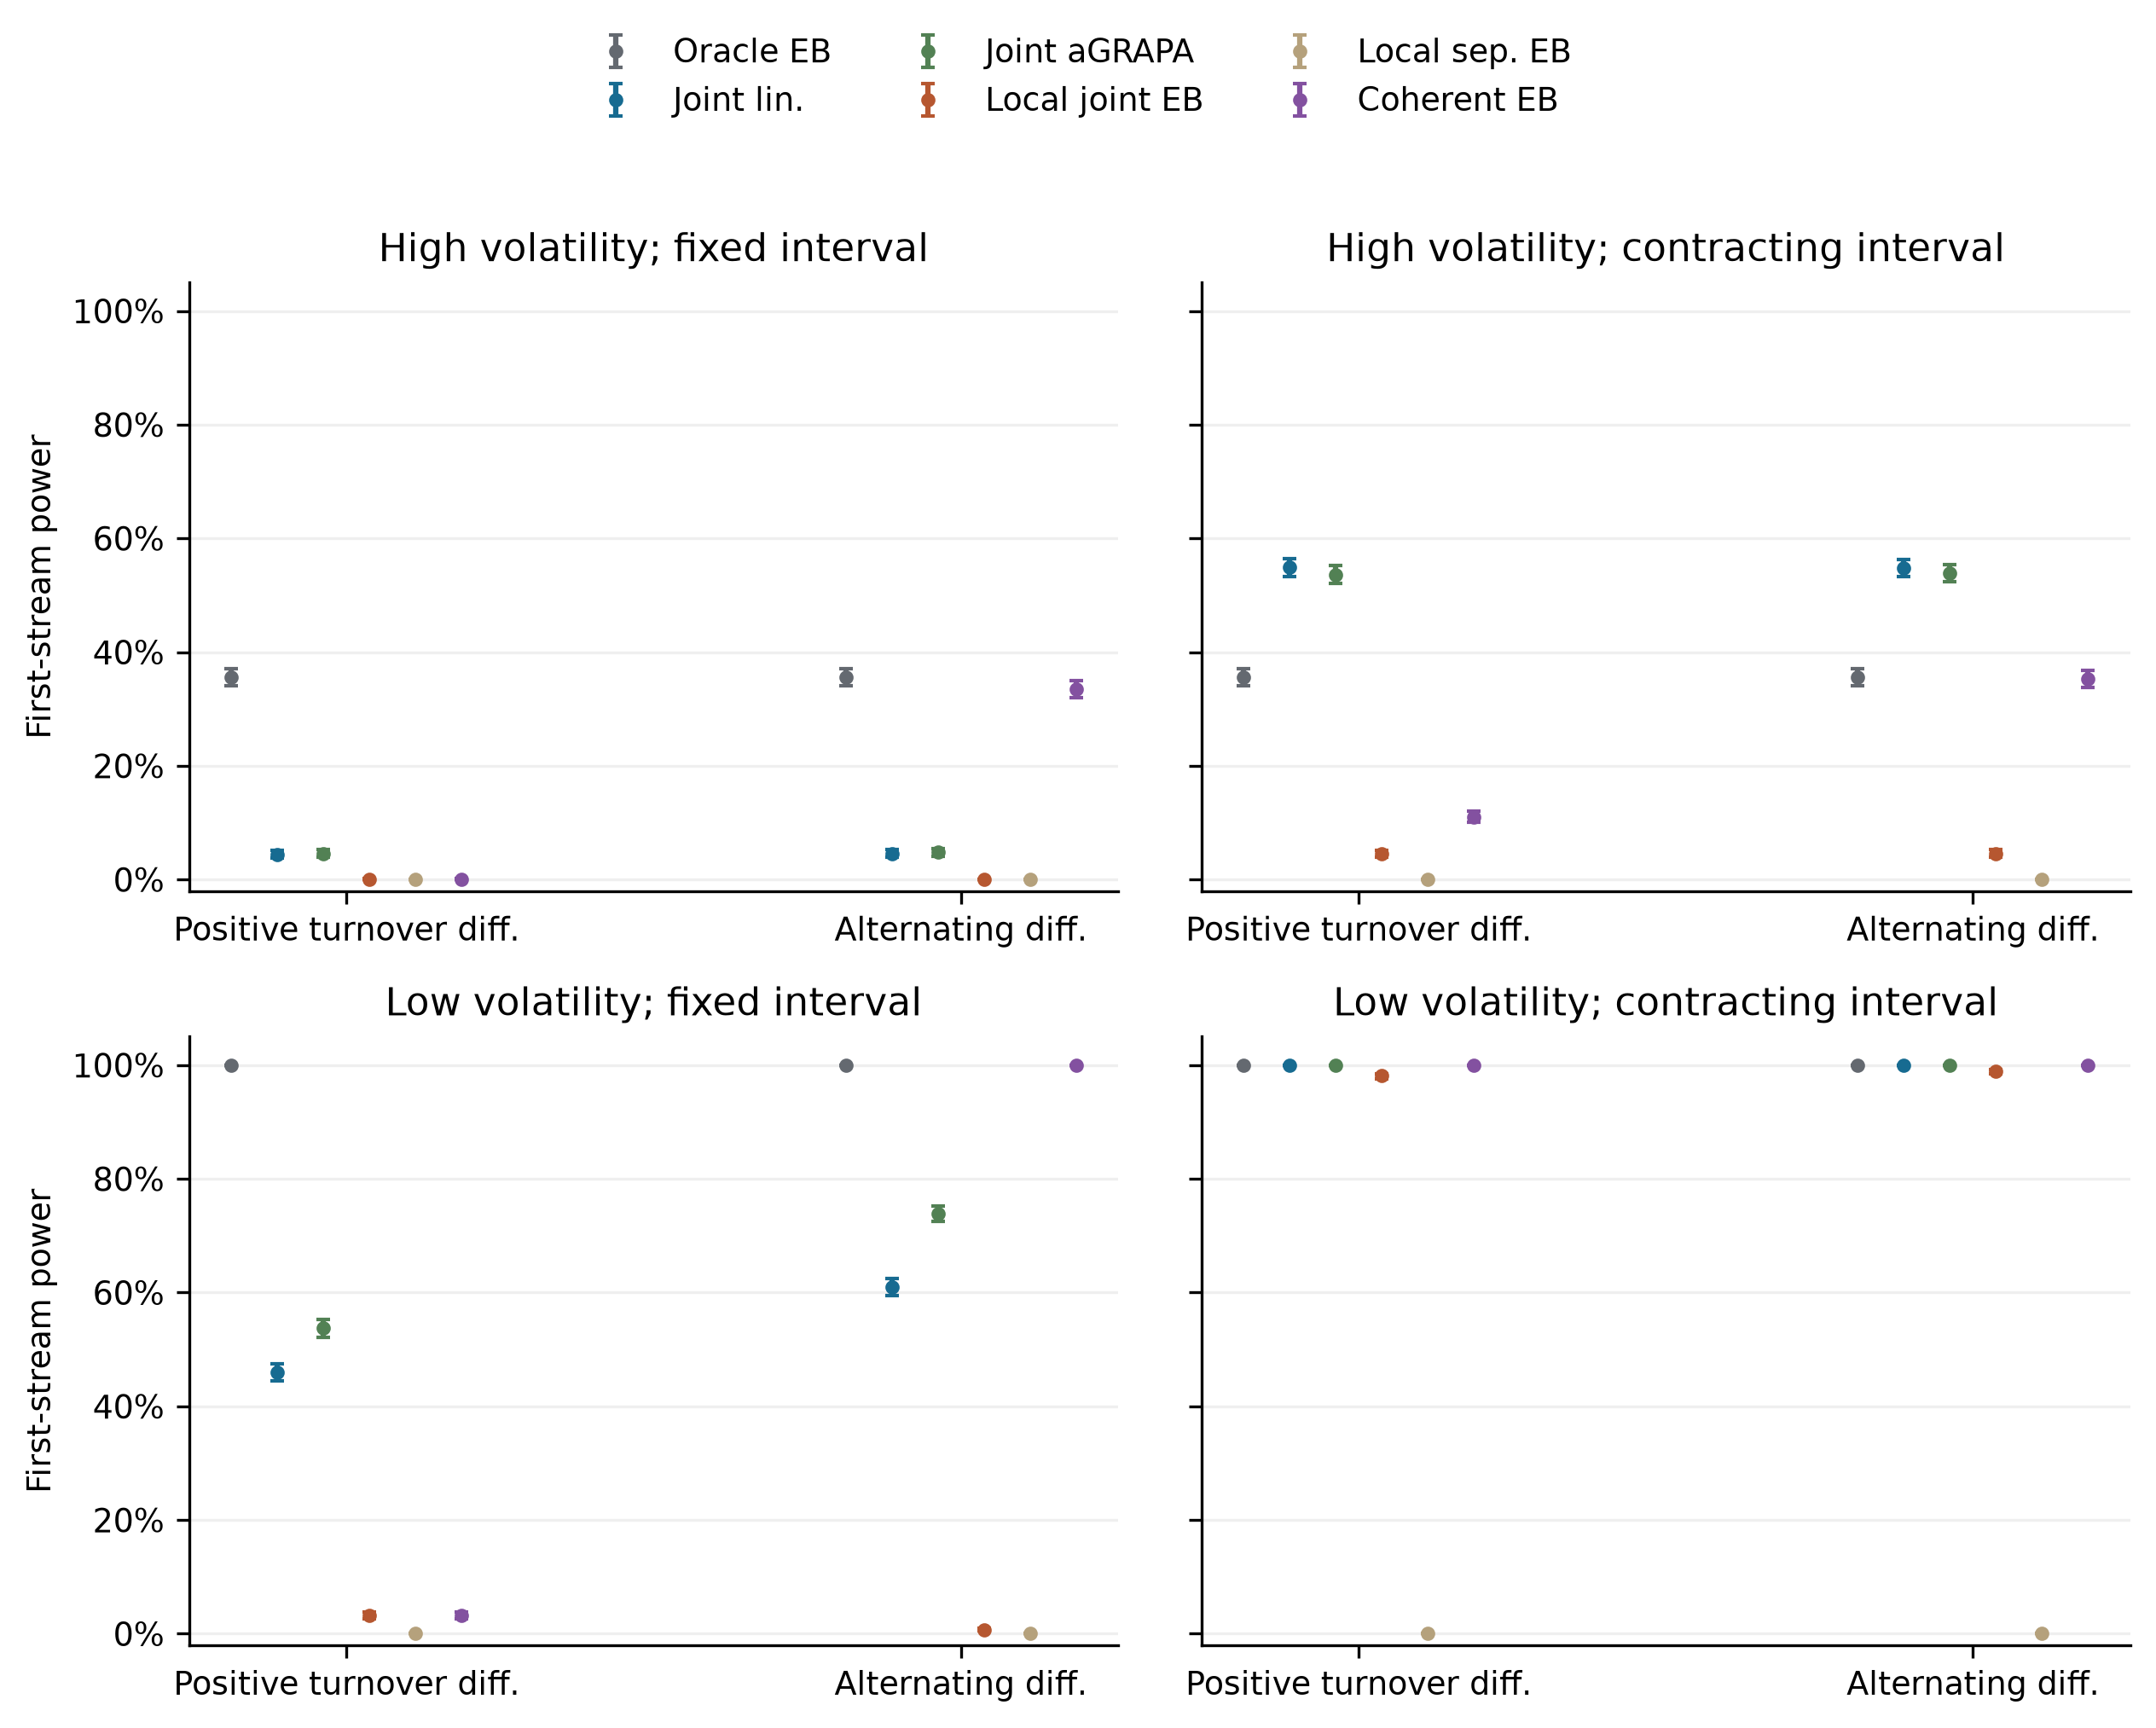
\includegraphics[width=\textwidth]{generated/followup/power.png}
\caption{Follow-up effect-0.05 factorial comparison. Points have within-case
95\% Wilson intervals over 4,000 worlds. Oracle EB knows the true cost;
its predictable centers match the other EB methods. Static and contracting
information use different calibration schedules. Factorial cells share seeded
innovations and must not be pooled as independent replications.}
\label{fig:followup-power}
\end{figure}

Temporal coherence does not make EB uniformly preferable to other evidence
forms. Under high volatility and contracting information, joint linear betting
has greater power than coherent EB, for both turnover patterns. Lower volatility
and sign changes can reverse that comparison. Likewise, the joint aGRAPA minus
joint linear power contrast ranges from \FollowupAgraGainMin\ to
\FollowupAgraGainMax\ percentage points across the eight primary cells. Its
negative high-volatility/contracting contrasts and positive low-volatility/static
contrasts rule out a uniform empirical advantage. Predictable refitting also
has a stronger conditional-null requirement than the fixed-grid comparisons.

Local joint versus local separate EB gains range from
\FollowupJointSeparateGainMin\ to \FollowupJointSeparateGainMax\ percentage
points. These are a different ablation from coherent versus local joint EB.
Both must be held separate from changing the underlying betting rule or the
cost-calibration schedule. The results identify mechanisms within the declared
synthetic family, rather than a universally best sequential procedure.

Weak effects remain difficult. Across the eight effect-0.02 cells, coherent EB
first-stream rejection never exceeds 1.825\%. The stronger effect-0.05 gains
therefore do not establish sensitive detection of small improvements at this
horizon, even inside the synthetic family.

\begin{table}[tb]\centering
\begingroup\small\setlength{\tabcolsep}{3pt}
\begin{tabular}{lrrr}\toprule
Case & aGRAPA - linear & Coherent - local EB & Joint - separate EB\\\midrule
F03 & 0.12 [-0.20, 0.45] & 0.00 $^{\ddagger}$ & 0.03 [-0.02, 0.07]\\
F06 & 0.18 [-0.15, 0.50] & 33.50 [32.04, 34.96] & 0.00 $^{\ddagger}$\\
F09 & -1.23 [-1.85, -0.60] & 6.48 [5.71, 7.24] & 4.50 [3.86, 5.14]\\
F12 & -0.88 [-1.50, -0.25] & 30.73 [29.30, 32.15] & 4.60 [3.95, 5.25]\\
F15 & 7.72 [6.90, 8.55] & 0.00 $^{\ddagger}$ & 3.20 [2.65, 3.75]\\
F18 & 12.90 [11.86, 13.94] & 99.30 [99.04, 99.56] & 0.70 [0.44, 0.96]\\
F21 & 0.00 $^{\ddagger}$ & 1.90 [1.48, 2.32] & 98.10 [97.68, 98.52]\\
F24 & 0.00 $^{\ddagger}$ & 1.10 [0.78, 1.42] & 98.90 [98.58, 99.22]\\
\bottomrule\end{tabular}
\endgroup
\caption{Prespecified effect-0.05 contrasts in first-stream power, in percentage points. Intervals are paired, approximate, unadjusted 95\% normal Monte Carlo intervals across worlds. $^{\ddagger}$ marks a degenerate sample with an unavailable normal interval, not known zero uncertainty. Case definitions appear in the supplement.}\label{tab:followup-paired}
\end{table}


\begin{figure}[tbp]\centering
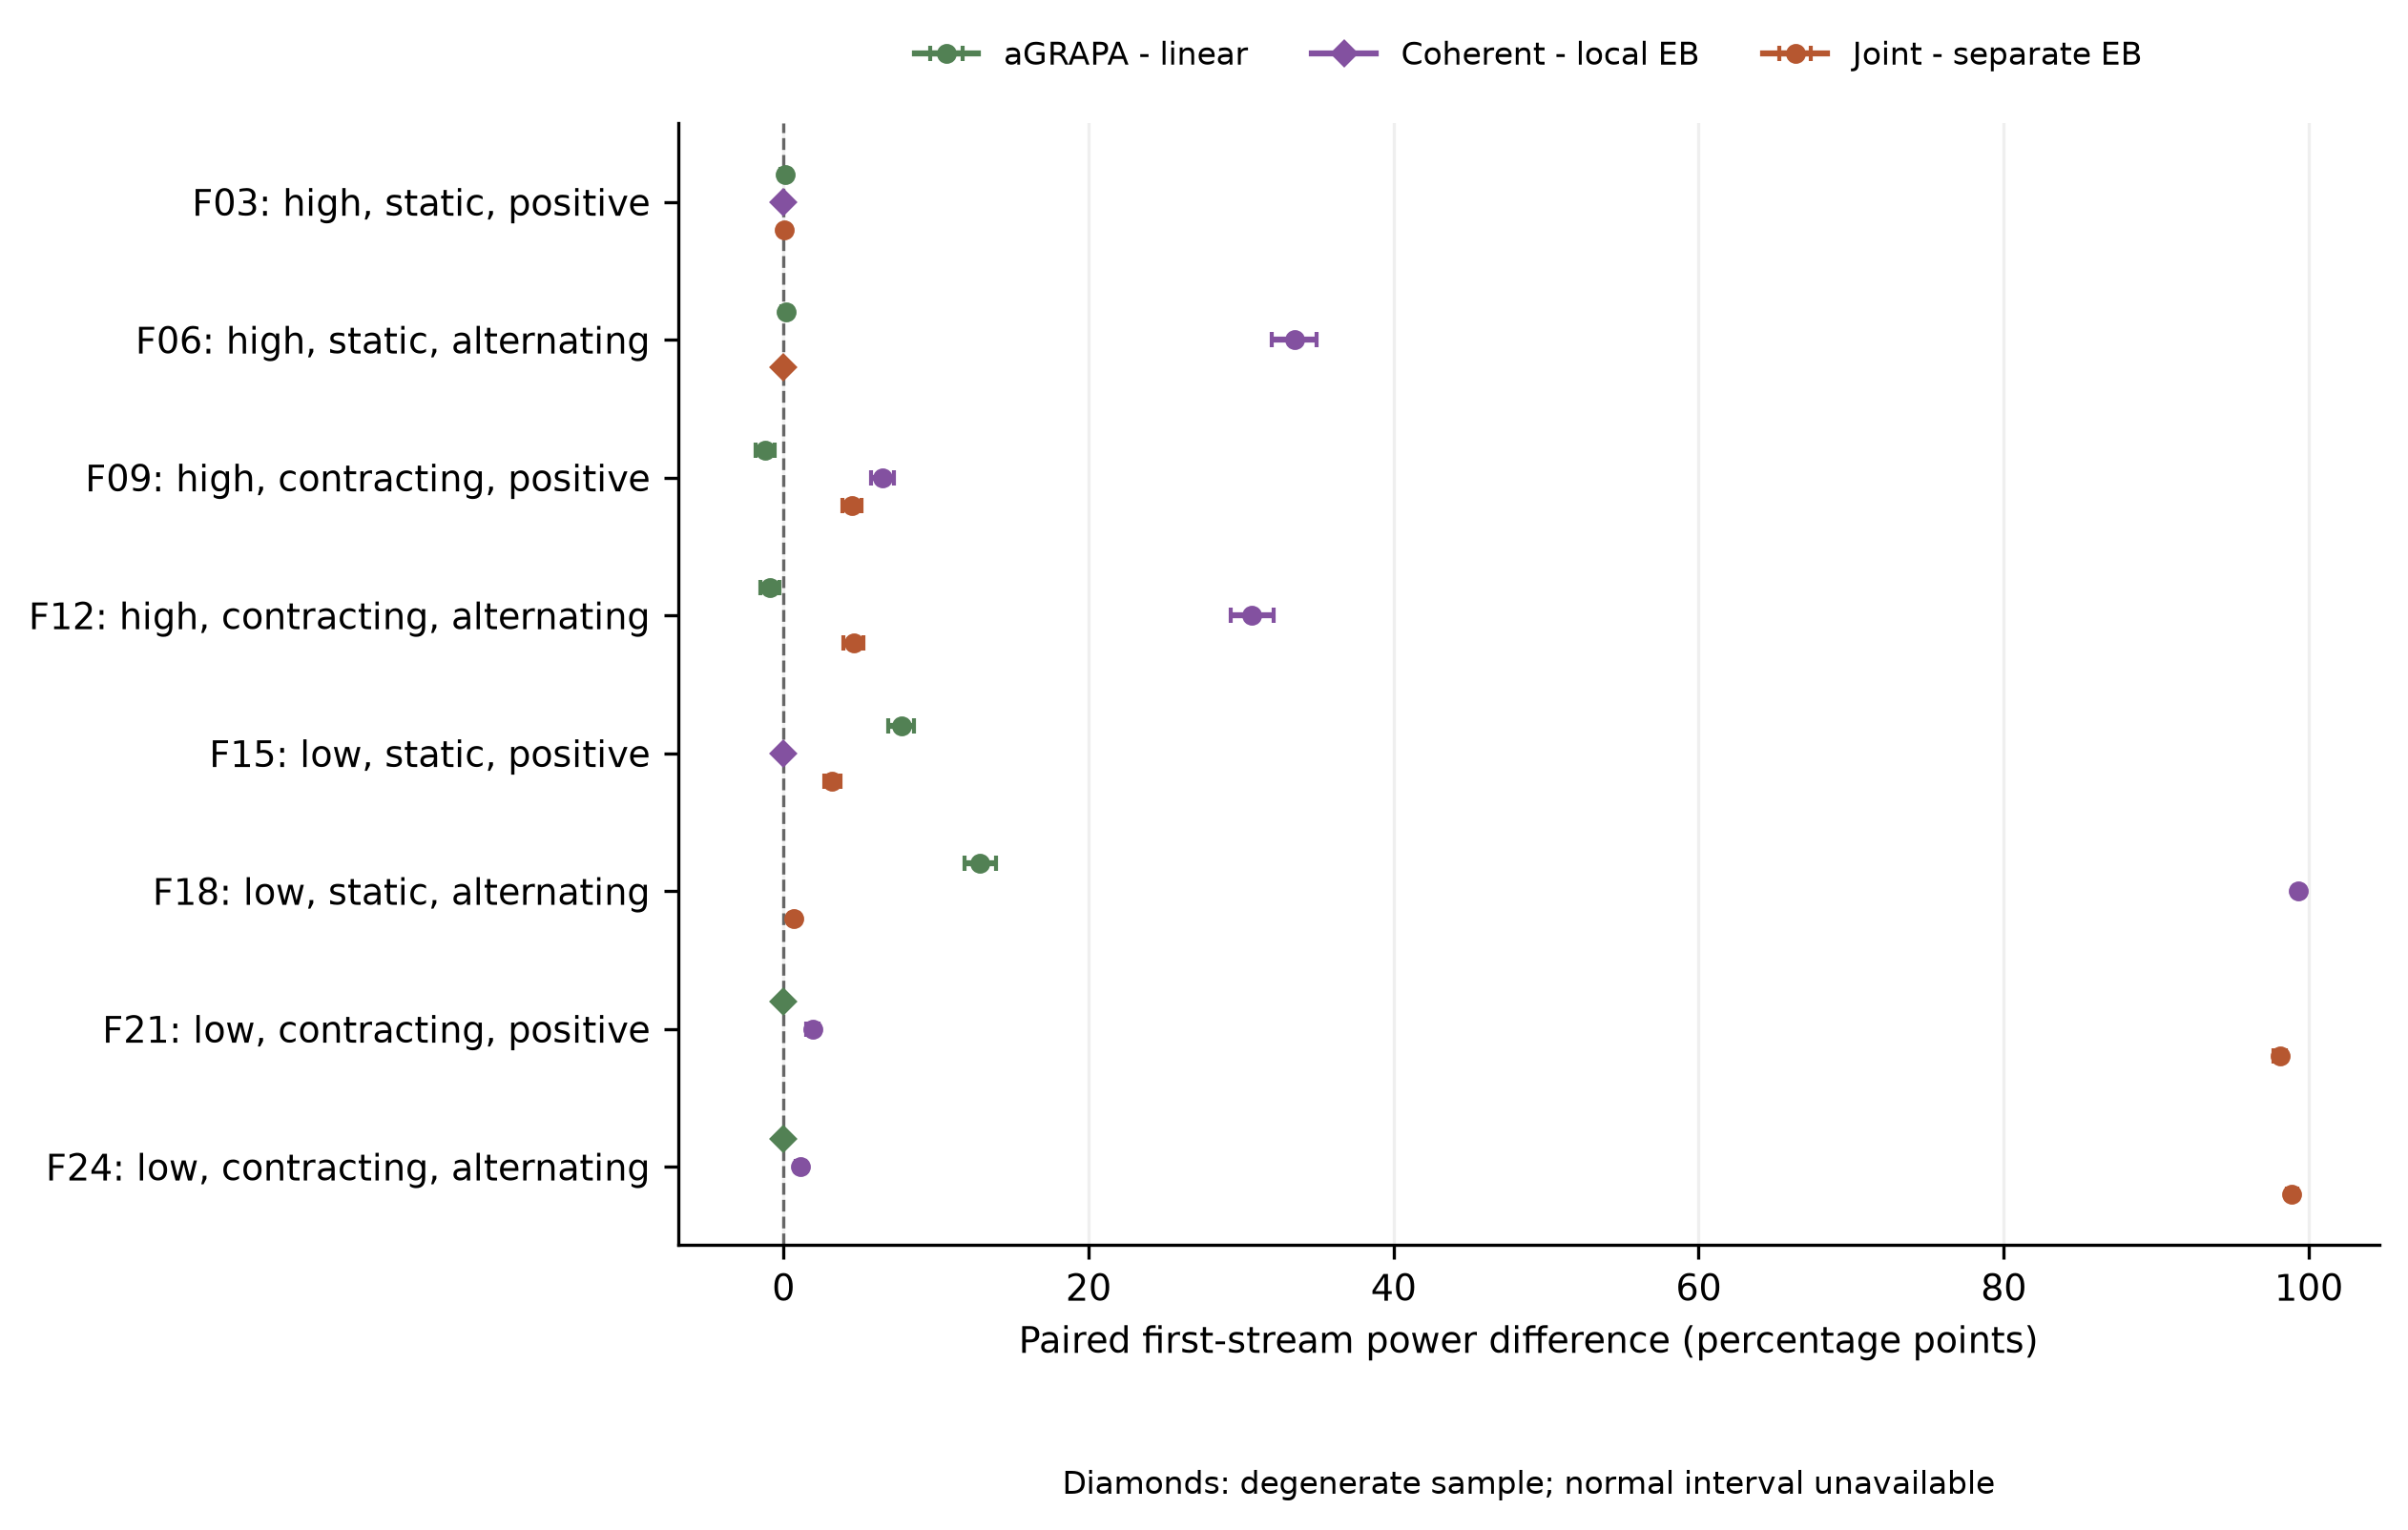
\includegraphics[width=\textwidth]{generated/followup/paired-power.png}
\caption{The three primary within-case ablations, with paired approximate
95\% normal Monte Carlo intervals. Intervals are unadjusted descriptive
summaries; diamonds denote degenerate samples for which that normal interval
is unavailable. Every registered contrast, including weaker effects, is
retained in the machine-readable supplement.}
\label{fig:followup-paired}
\end{figure}

Restricted detection time and subsequent paper utility follow the same
implementation's recorded allocation rule, not a funded portfolio. Saturated
end-of-horizon power does not imply identical detection times or utility;
those endpoints remain in the complete result tables. The prefix-weak diagnostic
has no first-stream rejections for any method. Its family rejection counts are
one for oracle linear, two for oracle aGRAPA and zero for the other methods,
out of 4,000 worlds each. These low frequencies do not validate aGRAPA
under that weaker null: Section~\ref{sec:followup-methods} gives its scope and
a deterministic counterexample to general predictable refitting.

Case kernels total 2,542.6 seconds on the recorded host. Named persistent state
uses 24,220,080 bytes per case; this is not peak process memory and runtime
excludes serialization. These observations describe reproducibility costs,
not controlled speed comparisons. All 250 method summaries, 150 paired
contrasts, calibration diagnostics and source-linked array outputs are retained.
